\documentclass[conference,a4paper]{IEEEtran}
\usepackage{cite}
\usepackage{amsmath,amssymb}
\usepackage{graphicx}
\usepackage{booktabs}
\usepackage{algpseudocode}

\graphicspath{{figures/}}

\begin{document}

\title{Sequential Training of Windowed Physics-Informed Neural Networks for the Lorenz-1960 Ordinary Differential Equation System}

\author{}

\maketitle

\begin{abstract}
We study a physics-informed neural network (PINN) approximation of a single nearly closed orbit of the Lorenz-1960 three-state system on the time interval from 0 to 13.26446. A single network trained on the full interval gives a combined state root-mean-square error (RMSE) of 2.237. To address this long-horizon problem, we divide the interval into 27 windows. Each window has a separate network and an initial state fixed to the predicted endpoint of the previous window. In each window, Adam reduces the residual in four stages using causal weights. Then, limited-memory Broyden–Fletcher–Goldfarb–Shanno (L-BFGS) minimizes the unweighted residual mean. A numerical reference monitors training but is not used for optimization or stopping. Across five seeds, the windowed model gives a median combined RMSE of 0.0000813 on 13,265 evaluation times. The seed-0 dense-grid residual mean square is 0.000000187. The full-interval and windowed runs differ in parameter count, sampling and optimizer schedule. Under the compared settings, separate window networks give lower final errors, while warm start improves accuracy and reduces Adam updates.

\end{abstract}

\begin{IEEEkeywords}
physics-informed neural network, Lorenz system, causal training, time windows, ordinary differential equation, windowed PINN
\end{IEEEkeywords}

\section{Introduction}
The Lorenz-system model is a three-state, nonlinear ordinary differential equation (ODE) obtained from a reduced flow model~\cite{lorenz1960}. Its initial-value problem provides a simple test of learning a continuous-time solution over a long interval. A physics-informed neural network (PINN) is trained with the ODE residual instead of solution samples~\cite{raissi2019}. Our goal is to find a training structure that approximates the full trajectory accurately. Long-horizon training is a known failure case of PINNs~\cite{wang2024causal,krishnapriyan2021}. We choose this system because numerical integration provides an accurate reference for evaluating the learned trajectory. Full-interval training couples early and late times, although the state at a later time depends on the preceding trajectory. Wang \emph{et al.} addressed this ordering with time-dependent residual weights~\cite{wang2024causal}. An initial condition can also be met by construction using a hard trial solution~\cite{lagaris1998}.

We use both concepts. We split the time period into 27 equal windows and use a separate network for every window. Each window starts from the predicted endpoint and copied parameters of the previous window. We report this implementation on $[0,13.26446]$, a nearly closed orbit for the chosen initial state, and compare it with a saved full-interval network. The comparison is descriptive because several configuration options differ. Our contributions are a windowed PINN with hard endpoint handoff, warm start and staged causal weights (Section~\ref{sec:windowed-pinn}); a five-seed evaluation with median combined root-mean-square error (RMSE) of $8.13\times10^{-5}$ against DOP853 (Section~\ref{sec:results}); and ablations showing lower final errors with separate networks and lower training cost with warm start under the compared settings (Section~\ref{subsec:ablation-results}).



\section{Problem and Background}
In this section we describe the Lorenz equations and the initial value problem that we want the model to learn. Then we explain the existing methods or components that we used.

\subsection{Lorenz Equations}
Our main object is a three-state nonlinear ordinary differential equation (ODE) that we need to solve. The system is non-chaotic and periodic and the time range approximates the period of a single loop.  Here $x(t)$, $y(t)$ and $z(t)$ are the three states, and $\kappa$ and $\ell$ are the physical wavenumbers. We use $k$ only for the window index, which comes later. The general form of the Lorenz system~\cite{lorenz1960} is:
\begin{equation}
\begin{aligned}
\frac{dx}{dt}
  &= \kappa\ell
     \left(\frac{1}{\kappa^2+\ell^2}
           -\frac{1}{\kappa^2}\right)yz,\\
\frac{dy}{dt}
  &= \kappa\ell
     \left(\frac{1}{\ell^2}
           -\frac{1}{\kappa^2+\ell^2}\right)xz,\\
\frac{dz}{dt}
  &= \frac{\kappa\ell}{2}
     \left(\frac{1}{\kappa^2}
           -\frac{1}{\ell^2}\right)xy.
\end{aligned}
\label{eq:lorenz1960}
\end{equation}

Suppose the state vector is given by
\[
u(t)=[x(t),y(t),z(t)]^\mathsf{T}.
\]
 We set $\kappa=2$ and $\ell=1$ in~\eqref{eq:lorenz1960} and get the three coefficients.


% Physical wavenumbers: \kappa and \ell.
% Window index: k.
\[
\begin{aligned}
a_x&=2(1/5-1/4)=-1/10=-0.1,\\
a_y&=2(1-1/5)=8/5=1.6,\\
a_z&=(2/2)(1/4-1)=-3/4=-0.75.
\end{aligned}
\]

Using these coefficient values, we get the reduced system we used in this experiment.
\begin{equation}
\dot{x}=-0.1\,yz,\qquad \dot{y}=1.6\,xz,\qquad \dot{z}=-0.75\,xy,
\label{eq:ode}
\end{equation}

If we collect the three right-hand sides, we get the vector form $du/dt=f(u)$. Here $f$ is the known ODE vector field.
\[
f(u)=[a_x yz,\,a_y xz,\,a_z xy]^\mathsf{T},\qquad f:\mathbb{R}^{3}\to\mathbb{R}^{3}.
\]

The input of $f$ is a state vector $u$ with three components and the output is the rate of change of $x$, $y$ and $z$ in the same order. While training, we use this same function on the predicted state $\hat{u}_k(t)$.

For our experiment we used the coefficients
\[
a=[a_x,a_y,a_z]^\mathsf{T}=[-0.1,1.6,-0.75]^\mathsf{T}.
\]
 The system starts from an initial state~\cite{matthews2024pinnde} of $u(0)=[0.5,0.75,1.0]^\mathsf{T}$ until a final time of $T=13.26446$. At this endpoint, the reference trajectory nearly returns to its starting state. It is very similar but not exactly closed so we call this interval a nearly closed orbit and not an exact period.


\subsection{Related Work}
In this study we investigate a combination of established concepts. A PINN embeds the physics residual into the training objective~\cite{raissi2019}. We use a hard trial-function design~\cite{lagaris1998} to fix the starting state exactly. Learning long trajectories is challenging because of the ordering of the time axis, which motivates causal residual weighting~\cite{wang2024causal}. Finally, timeline segmentation follows causal sweeping and temporal decomposition~\cite{penwarden2023}. We investigate these components on the nearly closed Lorenz-system orbit.

Several works explain why PINN training fails. Krishnapriyan \emph{et al.} studied failure modes and used sequence-to-sequence training~\cite{krishnapriyan2021}. Wang \emph{et al.} analyzed gradient imbalance and loss convergence through the neural tangent kernel~\cite{wang2021gradient,wang2022ntk}. For dynamical systems, fixed points can attract training toward an incorrect solution~\cite{rohrhofer2023}. Rathore \emph{et al.} found that Adam followed by limited-memory Broyden--Fletcher--Goldfarb--Shanno (L-BFGS) performed better than Adam alone on their PINN benchmarks~\cite{rathore2024}. Mattey and Ghosh retrained one network over successive segments while constraining it to retain earlier solutions~\cite{mattey2022bcpinn}. Our shared-network control does not include that backward-compatibility constraint.

\section{Windowed PINN}
\label{sec:windowed-pinn}

This section describes the network, hard initial conditions, causal loss and sequential training procedure.

\subsection{Network Structure}
We used several modeling strategies to approximate the solution for the Lorenz-system trajectory over $[0,T]$, where $T=13.26446$ is one nearly closed loop for the chosen initial state. We first tried one network to learn the entire trajectory at once. After the full-interval run reached a training plateau, we split the interval into equal segments.

Fig.~\ref{fig:plateau} shows the saved full-interval result.

\begin{figure}[t]
\centering
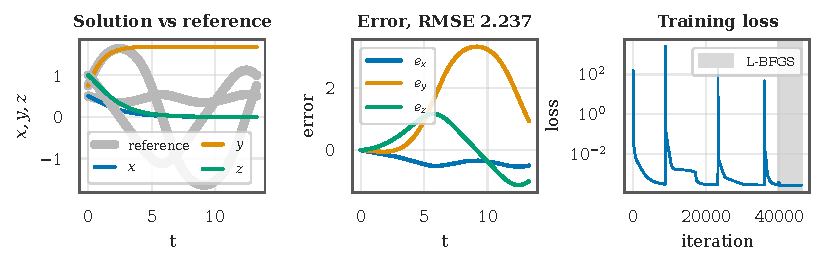
\includegraphics[width=\columnwidth]{figures/plateau-results.pdf}
\caption{Full-interval network: small residual, large trajectory error}
\label{fig:plateau}
\end{figure}

We chose a window width close to 0.5. Training one network sequentially over 27 windows gave final RMSEs of 0.350 to 0.648 over three seeds (Table~\ref{tab:ablations}). We therefore use a windowed PINN (WPINN), with a separate network for each window. Here $k=0,\ldots,26$ indexes the windows and $t_0,\ldots,t_{27}$ are the 28 boundary times. Each window $W_k$ has width $\Delta t=T/27$ and its own network parameters $\theta_k$.
\[
\begin{aligned}
t_k&=kT/27,\quad k=0,\ldots,27,\quad W_k=[t_k,t_{k+1}],\\
\Delta t&=T/27\approx0.4912763,\quad N_k(\,t;\theta_k):W_k\to\mathbb{R}^{3}.
\end{aligned}
\]


Each window has its own network $N_k(t;\theta_k)$ with one input ($t$), four hidden layers of 60 neurons with tanh units, and an output layer with 3 outputs. The output is a correction vector rather than the state $(x,y,z)$ directly. We get the predicted state $\hat{u}_k(t)$ from the trial solution in~\eqref{eq:trial}. With biases, the input layer has 120 parameters, the three hidden-to-hidden layers have $3\times3660$ and the output layer has 183. The total parameter count includes all 27 networks.
\[
P_{\mathrm{window}}=120+3(3660)+183=11{,}283,\; P_{\mathrm{total}}=304{,}641.
\]

For the model parameter initialization we used Xavier-uniform weights and zero biases. The 27 networks do not share parameters, but neighboring windows share a boundary. The predicted endpoint of a completed window is used as the initial state of the next window.

\subsection{Window Handoff}
As the Lorenz system is an initial value problem, we enforce the initial state of each window through a trial solution. Here $t_k$ is the starting time of window $k$, $u_{0,k}\in\mathbb{R}^3$ is its fixed starting state and $N_k(t;\theta_k)\in\mathbb{R}^3$ is the network raw output.
\begin{equation}
\begin{aligned}
\hat{u}_k(t)
  &=u_{0,k}+(t-t_k)N_k(t;\theta_k),\quad t\in W_k.
\end{aligned}
\label{eq:trial}
\end{equation}



At $t=t_k$, the second term is zero, so $\hat{u}_k(t_k)=u_{0,k}$ regardless of the network parameters~\cite{lagaris1998}. The first window uses the given initial state $u_{0,0}=u(0)$, and every later window uses the predicted endpoint of the last window as its initial state.
\begin{equation}
u_{0,k+1}=\hat{u}_k(t_{k+1}), \qquad k=0,\ldots,25.
\label{eq:handoff}
\end{equation}

The endpoint transfer in~\eqref{eq:handoff} and the trial solution make the predicted values continuous at the window boundaries. But the derivatives can still change suddenly at the boundaries. Window $k+1$ starts from a copy of the weights of window $k$, $\theta_{k+1}\leftarrow\theta_k$ for $k=0,\ldots,25$, and then trains its own parameters. As the starting point of the later windows is predicted, it can carry error from earlier windows.

Fig.~\ref{fig:pipeline} shows the implementation pipeline.

\begin{figure}[t]
\centering
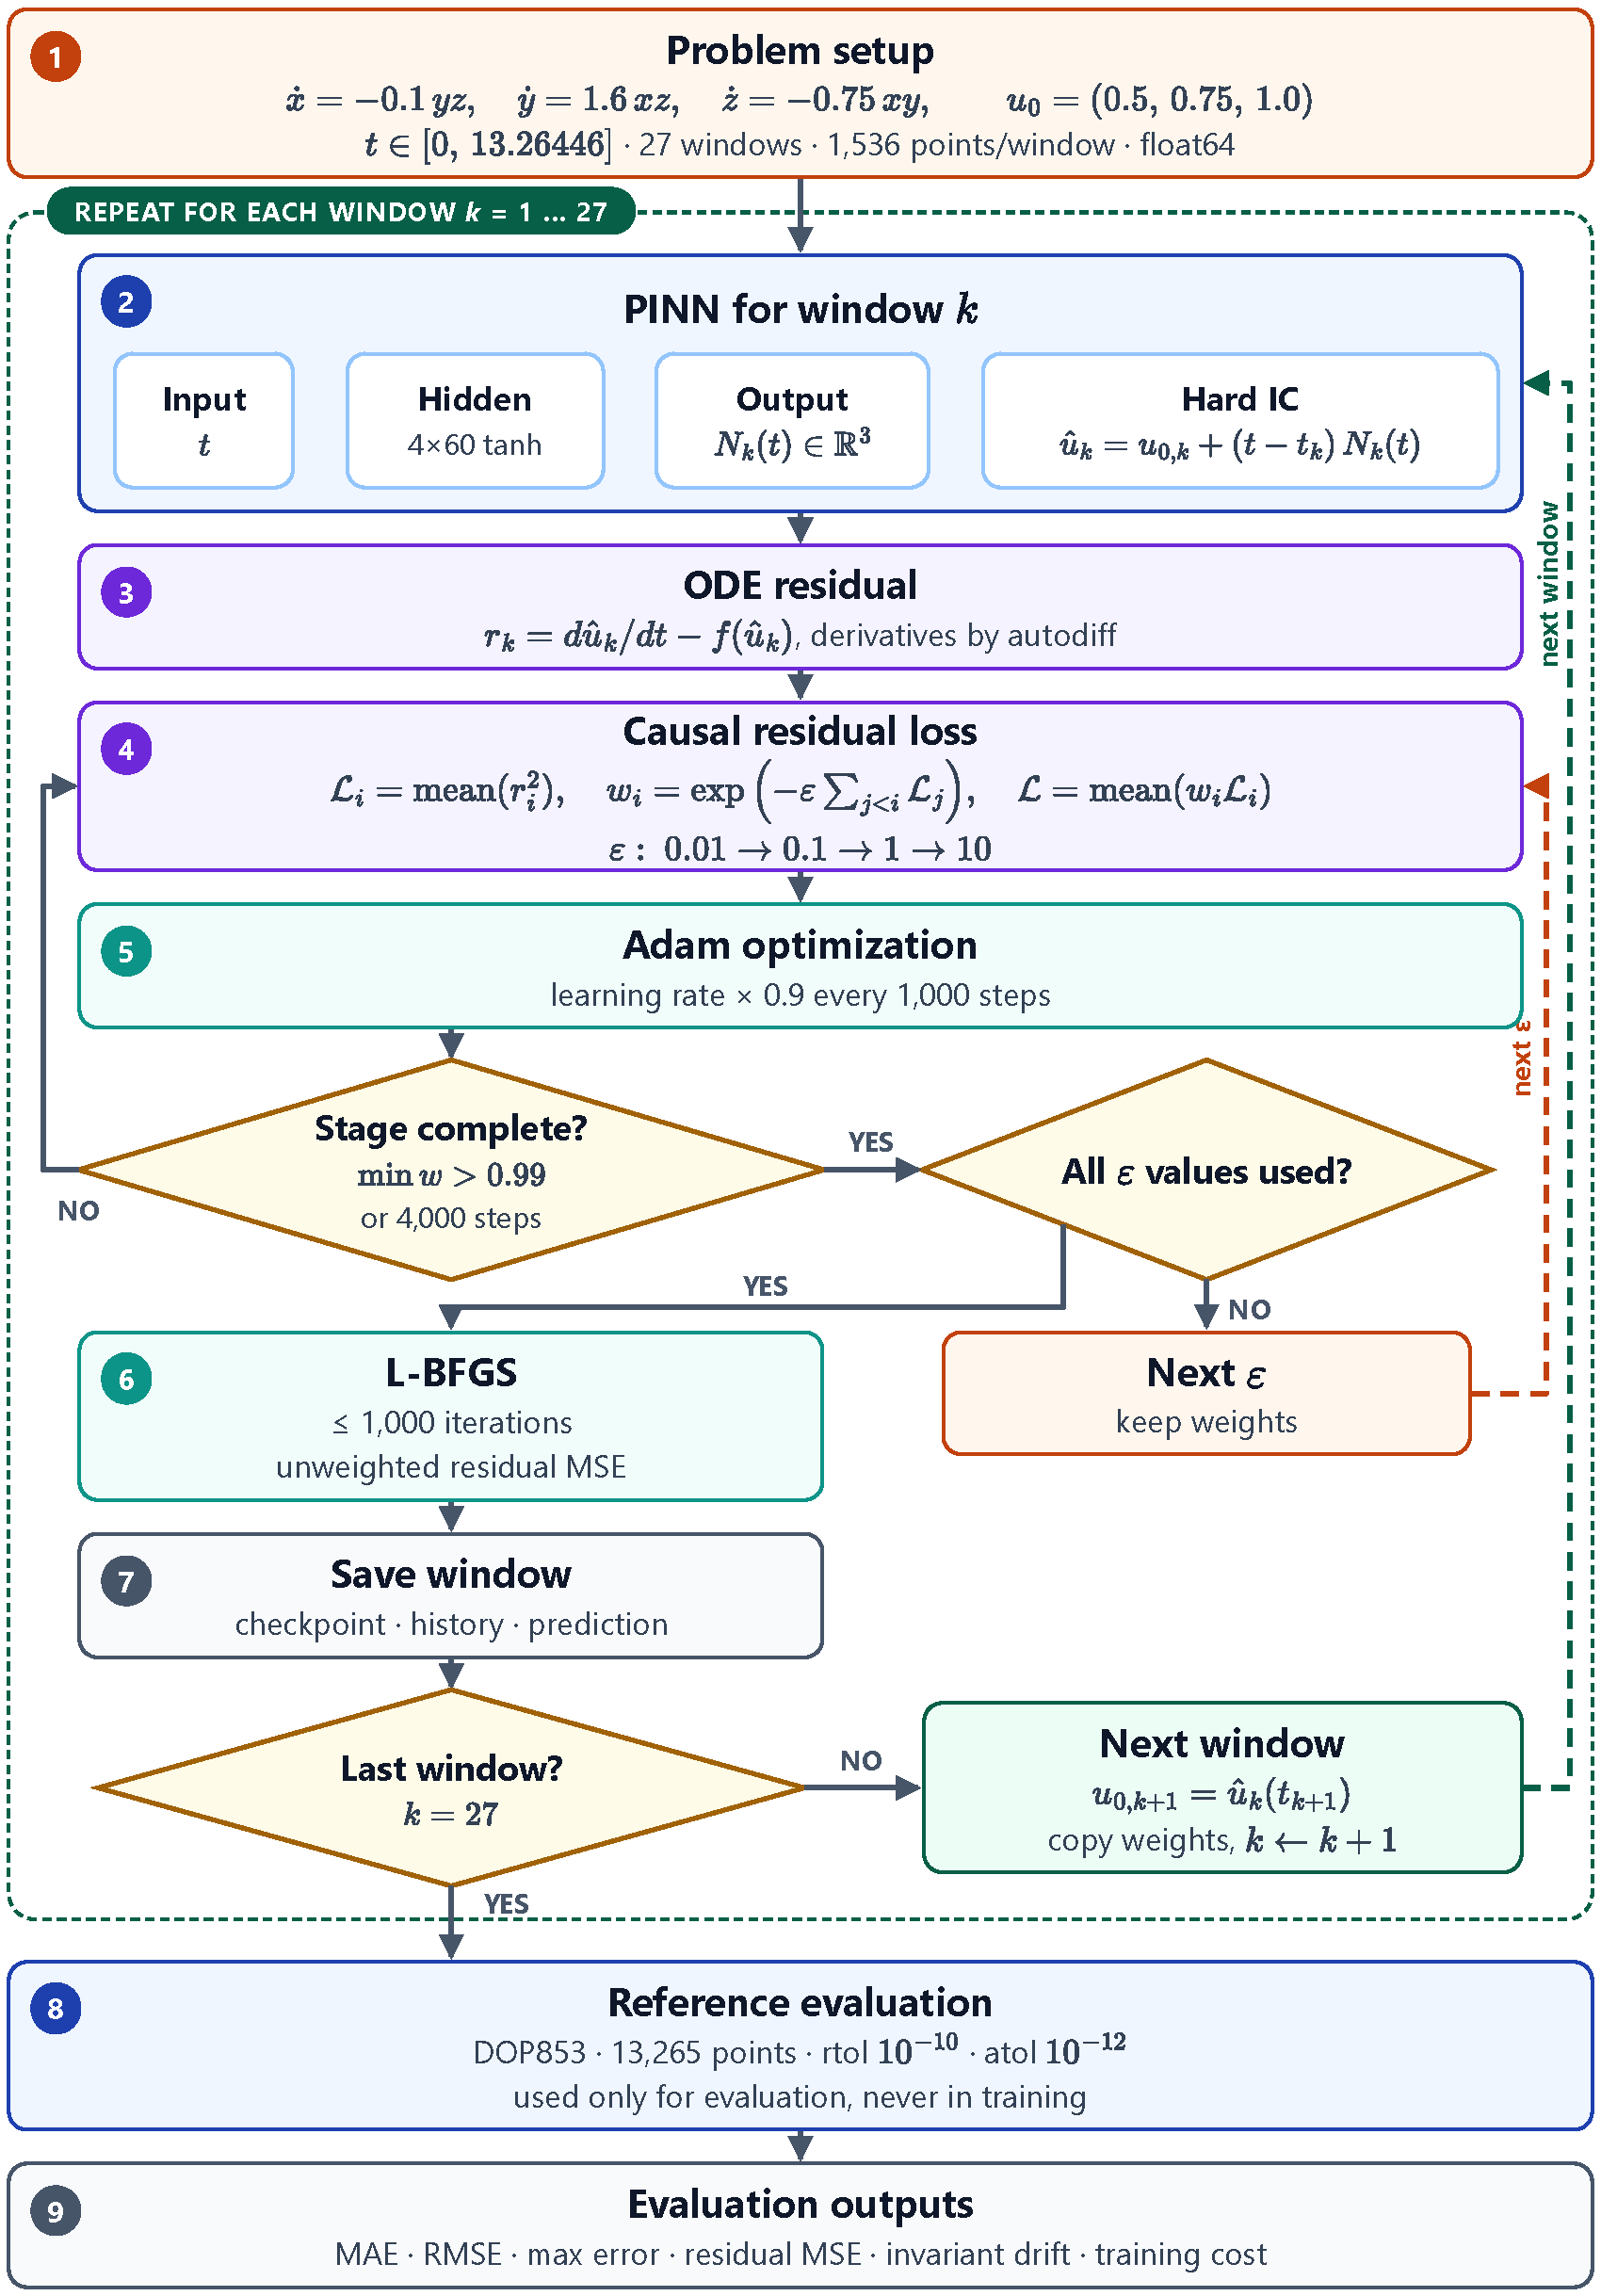
\includegraphics[width=\columnwidth]{figures/method.pdf}
\caption{Sequential training with endpoint handoff (windows 1--27)}
\label{fig:pipeline}
\end{figure}

\subsection{Training Loss}
To train the network of each window, we split the time range into $n_k=1536$ uniform collocation points $t_{k,i}$, $i=1,\ldots,n_k$, including both endpoints.
\[
\begin{aligned}
t_{k,i}&=t_k+\frac{i-1}{n_k-1}(t_{k+1}-t_k),\\
n_{\mathrm{unique}}&=27(1536-1)+1=41{,}446,\quad 27\cdot1536=41{,}472.
\end{aligned}
\]


Two windows next to each other share their boundary time. So there are 41,446 unique collocation points in total, but 41,472 collocation points are used in training. On the global grid, each boundary point belongs to the next window, and we also add it when we train the current window. The last window has the final endpoint. While training, all the points in a single window are passed to the network at once, which gives an output of shape $(1536,3)$.
Then we apply the trial solution to enforce the initial value. PyTorch automatic differentiation gives the rate of change of $x$, $y$ and $z$ with respect to time for all the collocation points. As $u_{0,k}$ is fixed while training, the product rule gives the derivative of~\eqref{eq:trial}:
\[
\frac{d\hat{u}_k}{dt}
=N_k+(t-t_k)\frac{\partial N_k}{\partial t}.
\]
% PyTorch autograd computes d\hat{u}_k/dt.
% f(\hat{u}_k) evaluates the prescribed ODE vector field.

The ODE residual function compares this derivative with $f(\hat{u}_k(t))$, which is the original ODE right-hand side at the predicted state. Both terms are vectors with three components, and their difference is the residual $r_k(t)$.
\begin{equation}
r_k(t)
=\frac{d\hat{u}_k(t)}{dt}
 -f\bigl(\hat{u}_k(t)\bigr)
\in\mathbb{R}^{3}.
\label{eq:residual}
\end{equation}
So the three components are $r_{k,x}=d\hat{x}_k/dt+0.1\,\hat{y}_k\hat{z}_k$, $r_{k,y}=d\hat{y}_k/dt-1.6\,\hat{x}_k\hat{z}_k$ and $r_{k,z}=d\hat{z}_k/dt+0.75\,\hat{x}_k\hat{y}_k$.

For a batch of $n_k$ times, each row is one collocation point and the three columns are $x$, $y$ and $z$. Here $\mathbf{N}_k$, $\hat{\mathbf{u}}_k$, $\dot{\hat{\mathbf{u}}}_k$, $\mathbf{f}_k$ and $\mathbf{r}_k$ mean the network outputs, trial states, time derivatives, ODE right-hand sides and residuals. Each of them is in $\mathbb{R}^{n_k\times3}$, and the time batch $\mathbf{t}_k$ is in $\mathbb{R}^{n_k\times1}$.
% Row i:
% \mathbf{N}_k: N_k(t_{k,i};\theta_k)^\mathsf{T}
% \hat{\mathbf{U}}_k: \hat{u}_k(t_{k,i})^\mathsf{T}
% \dot{\hat{\mathbf{U}}}_k: (d\hat{u}_k/dt)(t_{k,i})^\mathsf{T}
% \mathbf{F}_k: f(\hat{u}_k(t_{k,i}))^\mathsf{T}
% \mathbf{R}_k: r_k(t_{k,i})^\mathsf{T}

For each ordered collocation time $t_{k,i}$, we take the mean of the three squared residual components. This gives one non-negative loss value $L_{k,i}$ for each point instead of three components:
\begin{equation}
\begin{aligned}
L_{k,i}
  &=\tfrac{1}{3}\left\|r_k(t_{k,i})\right\|_2^2=\tfrac{1}{3}\bigl(r_{k,x}^2+r_{k,y}^2+r_{k,z}^2\bigr)(t_{k,i}).
\end{aligned}
\label{eq:pointloss}
\end{equation}

For a long-horizon, time-dependent ODE system, residual loss alone may not be sufficient. That is why we used causal weights and causal weighted loss. The causal weight at a time depends on the accumulated residual loss at earlier times~\cite{wang2024causal}. Here $S_{k,i}$ is the sum of the point losses at all earlier times of the same window. The first point has no earlier point, so $S_{k,1}=0$ and its causal weight is one.
\begin{equation}
w_{k,i}
=\exp\left(-\epsilon S_{k,i}\right)
=\exp\left(-\epsilon\sum_{j=1}^{i-1}L_{k,j}\right).
\label{eq:weights}
\end{equation}
So $0<w_{k,i}\leq1$. Then we multiply each point loss with its causal weight and take the mean over all $n_k$ points. This gives one loss value for the window in the current $\epsilon$ stage:
\begin{equation}
\mathcal{L}_{k,\epsilon}
=\frac{1}{n_k}
 \sum_{i=1}^{n_k}w_{k,i}L_{k,i}
\in\mathbb{R}_{\geq0}.
\label{eq:causalloss}
\end{equation}
% k: window index; i: current point; j: earlier point.
% \epsilon: scalar causal-weighting parameter.
% \mathcal{L}_{k,\epsilon}: one scalar objective at current parameters.
% Weights are recomputed, then detached for gradient calculation.

Here $k$ is the window, $i$ is the current point and $j<i$ means the earlier points of $i$. $\mathbf{L}_k,\mathbf{w}_k\in\mathbb{R}^{n_k}$ have one loss and one weight for each point. $\epsilon$ in the equation means how strongly the earlier losses reduce the later weights. We used four $\epsilon$ stages: $0.01$, $0.1$, $1$, and $10$. When the earlier losses go down, the later weights go up towards one. The weights are recomputed during training, and they are fixed while the Adam optimizer calculates the gradient. The causal weights also depend on the number and spacing of the collocation points~\cite{wang2024causal}.

On long intervals, a small residual can coexist with a large trajectory error. Causal weights reduce the influence of later points until earlier residuals are small. Equations~\eqref{eq:pointloss}--\eqref{eq:causalloss} define these point losses and weights. The next subsection gives the stage stopping rules and unweighted L-BFGS refinement.

\subsection{Training Procedure}

The causal loss defined above is minimized separately in each window. Fig.~\ref{fig:pipeline} summarizes the sequence across the windows. Fig.~\ref{fig:training} gives the training steps. In each window, an Adam optimizer and a StepLR scheduler are created. The learning rate starts at $10^{-3}$ and it is multiplied by 0.9 for every 1,000 updates across all four $\epsilon$ stages of the window. There is a 4,000 update limit for each stage. After every Adam update the code recalculates the causal weights at all collocation points of the window. If the minimum causal weight of all 1536 points of the window is above 0.99 after an update, then it moves to the next $\epsilon$ stage. If it is below 0.99 and it reaches the update limit then it moves to the next stage and records that the stage was capped.

When all four stages are completed, L-BFGS minimizes the unweighted residual mean for up to 1,000 iterations. For L-BFGS, we remove the causal weights and use the plain mean of the point losses.
\[
\mathcal{L}^{\mathrm{raw}}_k
=\frac{1}{n_k}\sum_i L_{k,i}
=\frac{1}{3n_k}\sum_i\|r_k(t_{k,i})\|_2^2.
\]

The reported seed-0 run uses a snapshot interval of 2,000 updates. After each window, we store its trained parameters and predicted endpoint. The same parameters initialize the next window. Reference values are used only for evaluation. After training, we measure errors and residuals on the collocation and evaluation grids.

\begin{figure}[t]
\centering
\begin{minipage}{\columnwidth}
\begin{algorithmic}[1]
\Require Ordered windows $W_0,\ldots,W_{26}$ and their uniform time points
\State Set $u_{0,0}\gets[0.5,0.75,1.0]^\mathsf{T}$
\For{$k=0,\ldots,26$}
  \If{$k>0$}
    \State Set $u_{0,k}\gets\hat{u}_{k-1}(t_k)$
    \State Initialize $\theta_k\gets\theta_{k-1}$
  \EndIf
  \State Add $t_{k+1}$ to the residual points if $k<26$
  \For{$\epsilon\in(0.01,0.1,1,10)$}
    \For{at most 4,000 Adam steps}
      \State Use ordered times $t_{k,i}$, $i=1,\ldots,n_k$
    \State Form $\hat{u}_k$ by~\eqref{eq:trial}; get $d\hat{u}_k/dt$ by autograd
    \State Form $r_k$ by~\eqref{eq:residual} and $L_{k,i}$ by~\eqref{eq:pointloss}
    \State Compute $w_{k,i}$ by~\eqref{eq:weights}; detach weights
      \State Backpropagate~\eqref{eq:causalloss}; Adam then StepLR
      \If{verified post-update $\min_i w_{k,i}>0.99$}
        \State \textbf{break}
      \EndIf
    \EndFor
    \State Record whether the threshold was met or capped
  \EndFor
  \State Run L-BFGS on the unweighted residual loss
  \State Save window model, endpoint state, and config record
\EndFor
\end{algorithmic}
\end{minipage}
\caption{Sequential window training}
\label{fig:training}
\end{figure}

\begin{table*}[t]
\caption{Ablation results (medians over seeds)}
\label{tab:ablations}
\centering\footnotesize
\begin{tabular}{lcccc}
\toprule
Configuration & Seeds & Median RMSE & RMSE range & Residual MSE\\
\midrule
WPINN & 5 & $8.13\!\times\!10^{-5}$ & $6.97\!\times\!10^{-5}$--$2.60\!\times\!10^{-4}$ & $1.87\!\times\!10^{-7}$\\
No causal & 3 & $1.89\!\times\!10^{-4}$ & $1.75\!\times\!10^{-4}$--$5.16\!\times\!10^{-4}$ & $8.81\!\times\!10^{-7}$\\
No warm start & 3 & $2.85\!\times\!10^{-4}$ & $1.76\!\times\!10^{-4}$--$2.88\!\times\!10^{-4}$ & $8.35\!\times\!10^{-7}$\\
Shared network & 3 & $0.486$ & $0.350$--$0.648$ & $0.965$\\
Causal single & 1 & $0.275$ & -- & $5.23\!\times\!10^{-6}$\\
Full interval & 1 & $2.237$ & -- & $2.80\!\times\!10^{-4}$\\
\bottomrule
\end{tabular}
\end{table*}


\section{Experimental Setup}

This section gives the saved run's configuration, reference and evaluation measures. The analysis uses saved configurations and checkpoints; the historical uncommitted source diff was not retained.

\subsection{Reference Solution}


Table~\ref{tab:config} shows the parameters used for the reported windowed run. We use SciPy’s DOP853~\cite{virtanen2020} as the numerical reference, a relative tolerance of $10^{-10}$ and an absolute tolerance of $10^{-12}$. It is sampled at 13,265 equally-spaced time points on a separate evaluation grid.

\begin{table}[t]
\caption{Windowed-run configuration}
\label{tab:config}
\centering\footnotesize
\begin{tabular}{ll}
\toprule
Setting & Value\\
\midrule
Interval; windows & $[0,13.26446]$; 27 equal windows\\
Network per window & $1$-$60$-$60$-$60$-$60$-$3$, tanh\\
Parameters & 11,283/window; 304,641 total\\
Initial condition; precision & $[0.5,0.75,1.0]^\mathsf{T}$; float64\\
Uniform collocation grid & 41,446 unique points\\
Adam $\epsilon$ stages & $0.01,0.1,1,10$\\
Stage threshold; steps/stage & $\min_{1\leq i\leq n_k}w_{k,i}>0.99$; 4,000\\
Adam rate; scheduler & $10^{-3}$; $\times0.9$ per 1,000 steps\\
L-BFGS budget & at most 1,000 iterations/window\\
Warm start; seed & Initialize $\theta_k\gets\theta_{k-1}$; 0\\
Reference grid & 13,265 uniform times\\
\bottomrule
\end{tabular}
\end{table}

\subsection{Evaluation}
At each evaluation time $t_j$, $j=1,\ldots,n_{\mathrm{eval}}$, we subtract the reference state from the predicted state and get the error vector $e(t_j)\in\mathbb{R}^3$. This error is not the same as the ODE residual.
\[
\begin{aligned}
e(t_j)&=\hat{u}(t_j)-u_{\mathrm{ref}}(t_j)=[e_x,e_y,e_z]^\mathsf{T}(t_j).
\end{aligned}
\]
For the combined RMSE, we take the mean of the squared error norms over all evaluation times and then the square root. It is also equal to the square root of the sum of the three squared component RMSEs.
\begin{equation}
\begin{aligned}
\operatorname{RMSE}_2
  &=\left(
      \frac{1}{n_{\mathrm{eval}}}
      \sum_{j=1}^{n_{\mathrm{eval}}}
      \|e(t_j)\|_2^2
     \right)^{1/2}.
\end{aligned}
\label{eq:rmse}
\end{equation}
For each state $c\in\{x,y,z\}$ we also report mean absolute error (MAE), RMSE and the maximum absolute error. $E_{\mathrm{mean}}$ and $E_{\mathrm{max}}$ are the mean and the maximum of the error norm.

The dense-grid residual mean square error (MSE) is the average of the three residual components squared, averaged over the evaluation times. So it has a factor of $1/(3n_{\mathrm{eval}})$, but the combined state RMSE is not divided by three.
\[
\operatorname{MSE}_{r,\mathrm{eval}}
=\frac{1}{3n_{\mathrm{eval}}}\sum_{j=1}^{n_{\mathrm{eval}}}\|r(t_j)\|_2^2.
\]
 The comparison run uses the same network depth and width on the entire interval $[0,T]$, and we compare their final outputs.

\subsection{Ablation Protocol}
Table~\ref{tab:ablations} shows all 16 completed runs. They use the same initial state, coefficients, float64 precision, interval and DOP853 evaluation grid. WPINN uses seeds 0--4; seed 0 supplies Tables~\ref{tab:errors} and~\ref{tab:comparison}. No-causal, no-warm-start and shared-network runs use seeds 1--3; the causal-single and full-interval runs use seed 0. Without causal weights, each window uses 1,300 Adam steps (35,100 total), close to WPINN's mean of 34,768. Without warm start, we retain the WPINN schedule but do not copy the previous window's parameters. The shared-network case uses the no-causal schedule and reuses one network over all 27 windows, without a constraint to retain earlier solutions. The causal-single run uses the full-interval grid and budget: 39,793 Latin hypercube sampling (LHS) points, 40,000 Adam steps and at most 5,000 L-BFGS iterations. We compare Adam updates rather than wall time because hardware differs.

\subsection{Failure Cases}
We use the shared-network and causal-single runs as failure cases, judged by their final error against DOP853. All runs completed training; a large final error indicates a poor prediction, not an interrupted job. Reaching the 4,000-step stage cap is recorded separately. Table~\ref{tab:ablations} includes every completed seed without a success-based selection cutoff.


\section{Results}
\label{sec:results}



\subsection{Prediction Accuracy}
We compare the windowed PINN with SciPy's DOP853 reference. Across five seeds, the median combined RMSE is $8.13\times10^{-5}$ and the best is $6.97\times10^{-5}$ on 13,265 uniform evaluation times. Table~\ref{tab:errors} reports seed 0, whose maximum state-error norm is $3.09\times10^{-4}$. Fig.~\ref{fig:trajectory} shows its prediction and reference; the curves overlap at the plotted scale, with small error peaks near $t\simeq5$. In the state-norm row, the MAE entry is $E_{\mathrm{mean}}$, the RMSE is $\operatorname{RMSE}_2$ from~\eqref{eq:rmse}, and the maximum is $E_{\mathrm{max}}$.

\begin{table}[t]
\caption{Windowed-run error (seed 0)}
\label{tab:errors}
\centering\footnotesize
\begin{tabular}{lccc}
\toprule
State & MAE & RMSE & Maximum\\
\midrule
$x$ & $1.89\times10^{-5}$ & $2.74\times10^{-5}$ & $1.13\times10^{-4}$\\
$y$ & $2.94\times10^{-5}$ & $4.96\times10^{-5}$ & $2.88\times10^{-4}$\\
$z$ & $2.78\times10^{-5}$ & $4.05\times10^{-5}$ & $1.30\times10^{-4}$\\
State norm & $5.12\times10^{-5}$ & $6.97\times10^{-5}$ & $3.09\times10^{-4}$\\
\bottomrule
\end{tabular}
\end{table}

\begin{figure}[t]
\centering
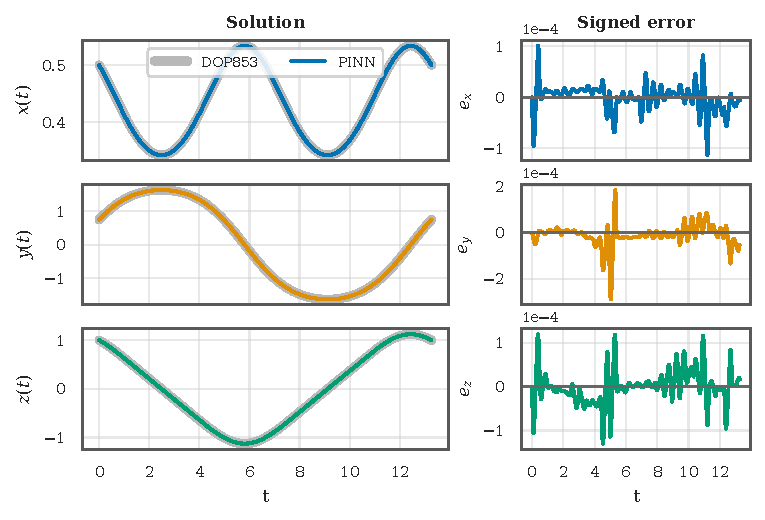
\includegraphics[width=\columnwidth]{figures/solution_vs_reference.pdf}
\caption{Windowed prediction follows DOP853 at the plotted scale (seed 0)}
\label{fig:trajectory}
\end{figure}

For seed 0, the residual MSE is $1.872\times10^{-7}$ on the evaluation grid and $1.874\times10^{-7}$ on the collocation grid. To check conservation in~\eqref{eq:ode}, let $b_1,b_2$ be the columns of SciPy's orthonormal null-space basis of $a^{\mathsf T}$. The two invariants are $I_i(t)=b_i^{\mathsf T}[x(t)^2,y(t)^2,z(t)^2]^{\mathsf T}$, $i=1,2$. For each, we report $\max_t|I_i(t)-I_i(0)|/|I_i(0)|$; both initial values are nonzero here. The maximum drift over the pair is below $4\times10^{-10}$ for DOP853 and $2.6\times10^{-4}$ for WPINN.

Lastly, the hard trial solution ensures that the state values are continuous at the inner 26 interfaces connecting the windows.


\subsection{Run Comparison}
Table~\ref{tab:comparison} compares the saved full-interval and seed-0 windowed runs. Their combined RMSEs are 2.237 and $6.97\times10^{-5}$. A small collocation residual does not guarantee an accurate trajectory~\cite{rohrhofer2023}. The configurations differ in causal weighting~\cite{wang2024causal}, windowing~\cite{penwarden2023}, warm start, sampling and optimizer budgets. WPINN also has 27 times as many parameters. The full-interval row in Table~\ref{tab:ablations} is the same saved run.

\begin{table}[t]
\caption{Full-interval and windowed runs}
\label{tab:comparison}
\centering\footnotesize
\begin{tabular}{lcc}
\toprule
Measure & One network & 27 windows\\
\midrule
Trainable parameters & 11,283 & 304,641\\
Training points & 39,793 LHS & 41,446 uniform\\
Combined state RMSE & 2.237 & $6.97\times10^{-5}$\\
Maximum state-error norm & 3.346 & $3.09\times10^{-4}$\\
Collocation residual MSE & $2.80\times10^{-4}$ & $1.87\times10^{-7}$\\
Recorded Adam steps & 40,000 & 34,765\\
\bottomrule
\multicolumn{3}{l}{LHS: Latin hypercube sampling.}\\
\end{tabular}
\end{table}

The 27 run windows had 34,765 Adam updates and 33,143 L-BFGS closure evaluations in total. Closure evaluations are function calls made by L-BFGS, not iterations. Only two of the 108 causal stages ended at the 4,000-step cap without meeting the $0.99$ weight threshold.

\subsection{Ablation and Failure Results}
\label{subsec:ablation-results}
Table~\ref{tab:ablations} shows the ablation results. WPINN has median RMSE $8.13\times10^{-5}$, with three of five seeds below $10^{-4}$. Without causal weights the median is about 2.3 times larger. An exact one-sided Mann--Whitney U test compares no-causal seeds 1--3 with WPINN seeds 0--4, testing for larger no-causal errors ($U=11$, $p=0.196$). This comparison is exploratory given the small groups and shared seed identifiers; seed 2 has lower error without causal weights. Without warm start, all three matched seeds have larger errors, mean Adam updates rise to 102,989, and 17--19 stages reach the cap, compared with 1--2 for WPINN. Reusing one network over the windows gives RMSEs of 0.350--0.648, compared with $1.75\times10^{-4}$--$5.16\times10^{-4}$ for separate networks under the same no-causal schedule. These final errors favor separate networks, but do not measure when earlier-window accuracy changes during training. The causal-single run gives RMSE 0.275. Together, the saved runs support the windowed training structure and the training-cost benefit of warm start for this orbit, without establishing a consistent accuracy gain from causal weighting.

\section{Conclusion}

Our 27-window PINN approximates the nearly closed Lorenz-system orbit on $[0,13.26446]$ with a five-seed median combined RMSE of $8.13\times10^{-5}$ against DOP853. The seed-0 RMSE is $6.97\times10^{-5}$, compared with 2.237 for the saved full-interval network. Separate window networks give lower final errors under the compared settings, and warm start reduces Adam updates while improving the matched-seed accuracy. This provides an effective training structure for the studied initial-value problem. Future work will test matched configurations, other initial states and coefficient sets to assess how well the approach extends beyond this orbit.








\section*{Acknowledgment}
Large language models were used only for non-intellectual assistance with formatting, typesetting, language editing and proofreading. The authors take responsibility for the manuscript's content and accuracy.

\bibliographystyle{IEEEtran}
\bibliography{references}

\end{document}
